\subsection{Рендеринг в Blender}

Blender поддерживает загрузку объемных данных в формате \texttt{.vdb}, в котором каждому вокселю можно приписать любое количество аттрибутов. Поэтому был написан скрипт по упаковке данных в этот формат, где:
%
\begin{itemize}
	\item \texttt{rgb}: отвечают 3 числа яркости каналов красного, зеленого и синего, переведенные $[0, 255] \cap \mathbb Z \to [0, 1]$;
	\item \texttt{ct}: аналогичное преобразование оттенков серого КТ;
\end{itemize}
%
Полный код конвертирования \texttt{.npy} (формат массивов numpy) в \texttt{.vdb} приведен в листинге \ref{lst:npy-to-vdb}.

Эти данные были загружены в Blender, к объемным данным применен шейдер (рис. \ref{fig:blender-shader}). Фазовая функция описывается здесь с помощью коэффициента анизотропии, где $1$ - рассеивание не меняет направление луча, $-1$ разворачивает его в противоположном направлении, промежуточные, $0$ - абсолютно случайное перенаправление. Конкретно для шейдера Principled Volume используется фазовая функция Хеньи-Гринштейна, но Blender поддерживает и другие, плотности (рис. \ref{fig:phase-functions}).

\begin{figure}[ht]
	\centering
	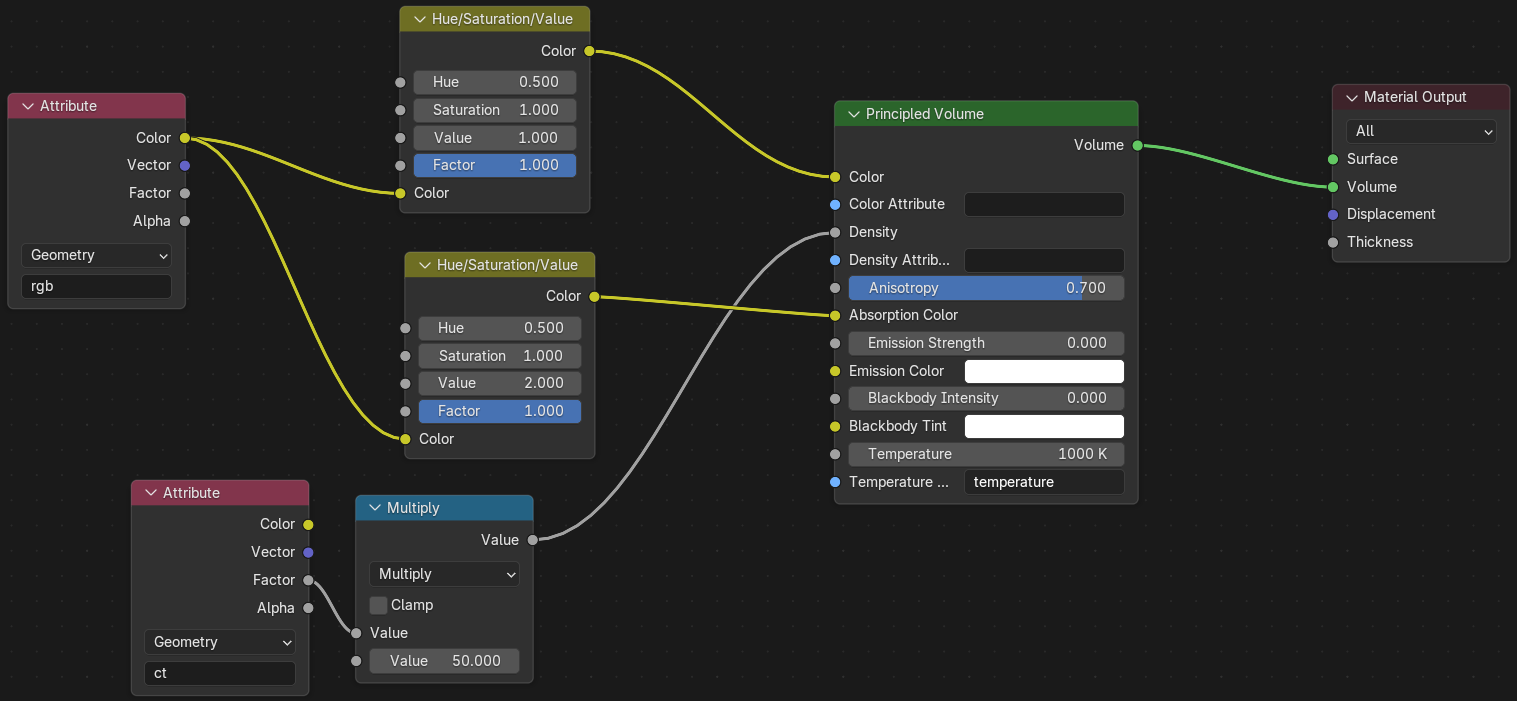
\includegraphics[width=\textwidth]{assets/blender_shader.png}
	\caption{Shader наложенный на загруженный в Blender объём; Absorption Color здесь --- это цвет, который выживает при поглощении; Color --- рассеиваемый цвет}
	\label{fig:blender-shader}
\end{figure}

\begin{figure}[ht]
	\centering
	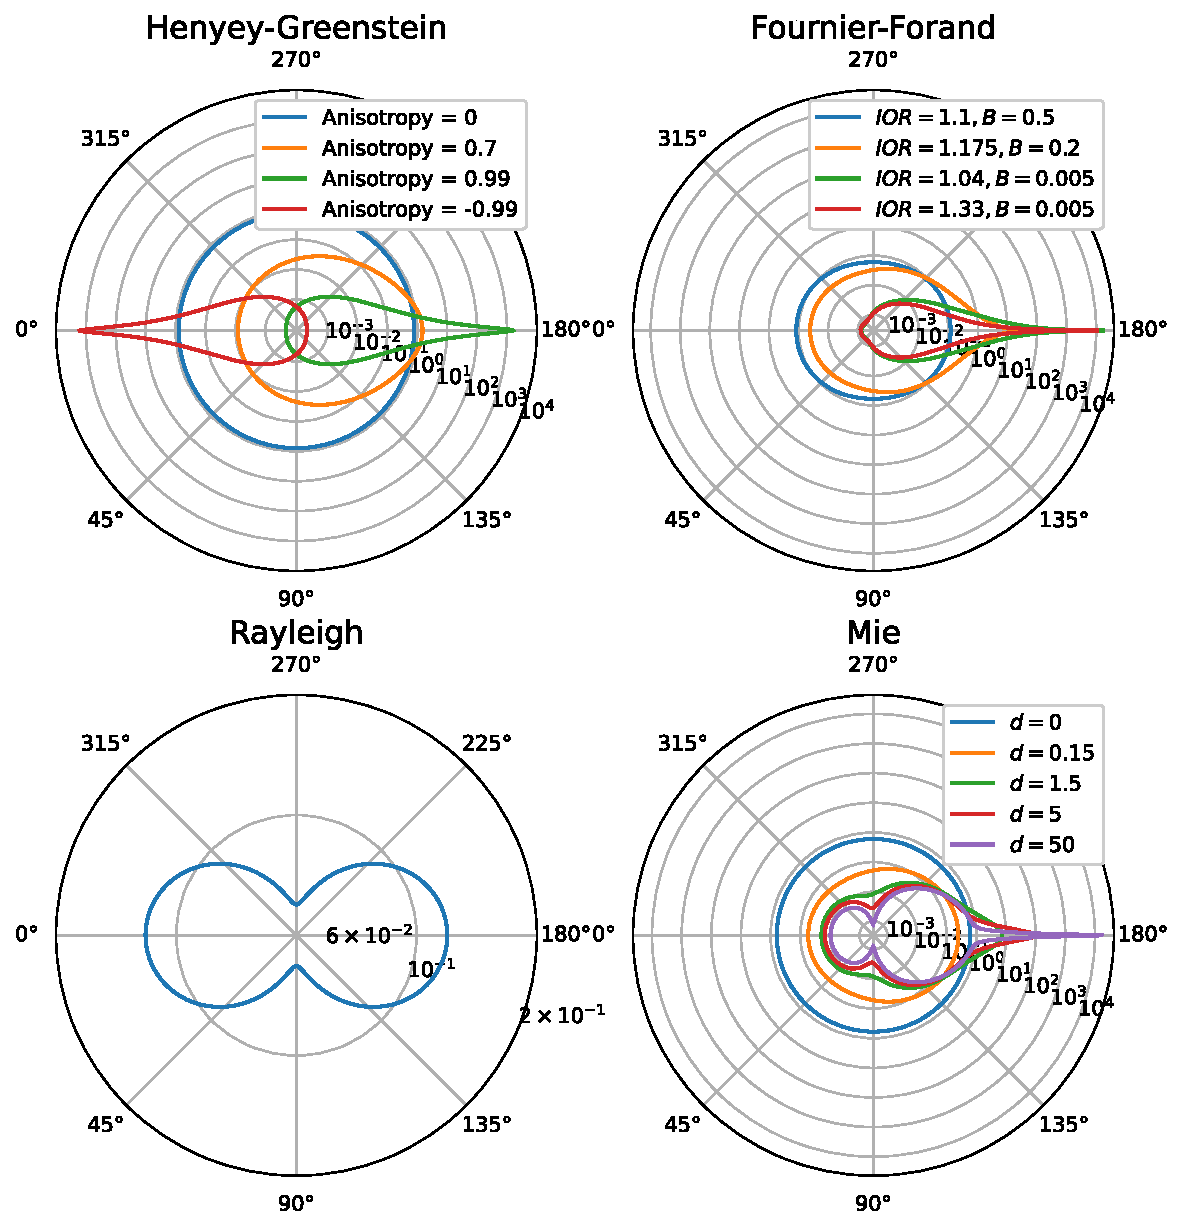
\includegraphics[width=0.5\textwidth]{assets/phase-functions.pdf}
	\caption{Плотности распределения фазовых функций из Blender при различных параметрах. Для функции Хеньи-Гринштейна им выступает анизотропия.}
	\label{fig:phase-functions}
\end{figure}

При загрузке объемных данных из формата \texttt{.vdb} воксель с координатами $(x, y, z)$ размещается ровно в таких же координатах Blender (рис. \ref{fig:load-vhp-blender}). Хотя сам формат поддерживает запись преобразований, которые надо произвести с вокселями, чтобы разместить их в нужном месте, приведенный ранее скрипт этого не учитывает, поэтому на объем наложены геометрические преобразования (рис. \ref{fig:blender-geometry}).

\begin{figure}[ht]
	\centering
	\begin{subfigure}[b]{0.49\textwidth}
		\centering
		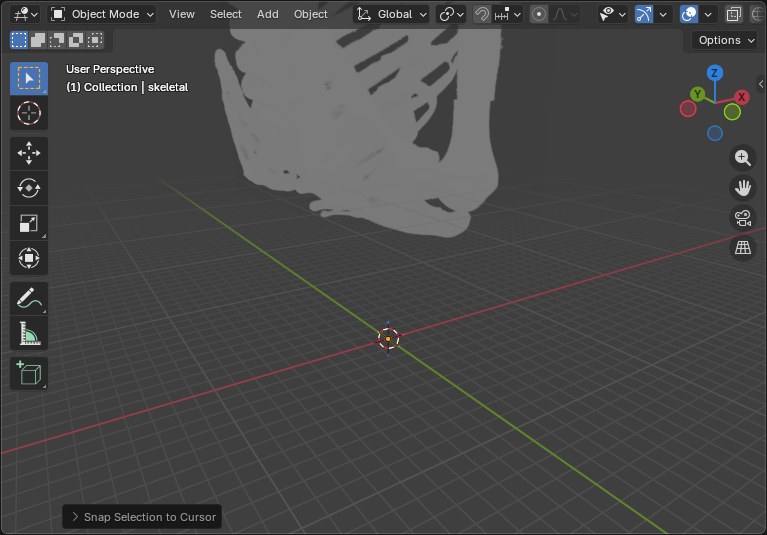
\includegraphics[width=\textwidth]{assets/before_geometry.png}
	\end{subfigure}%
	\hfill
	\begin{subfigure}[b]{0.49\textwidth}
		\centering
		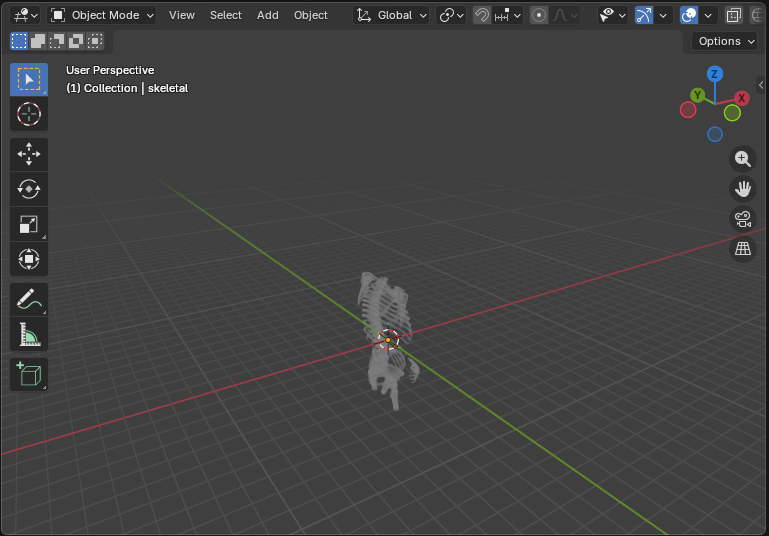
\includegraphics[width=\textwidth]{assets/after_geometry.png}
	\end{subfigure}%
	\caption{Слева изображено как выглядят загруженные в Blender данные в сыром виде, справа --- после преобразований}
	\label{fig:load-vhp-blender}
\end{figure}

\begin{figure}[ht]
	\centering
	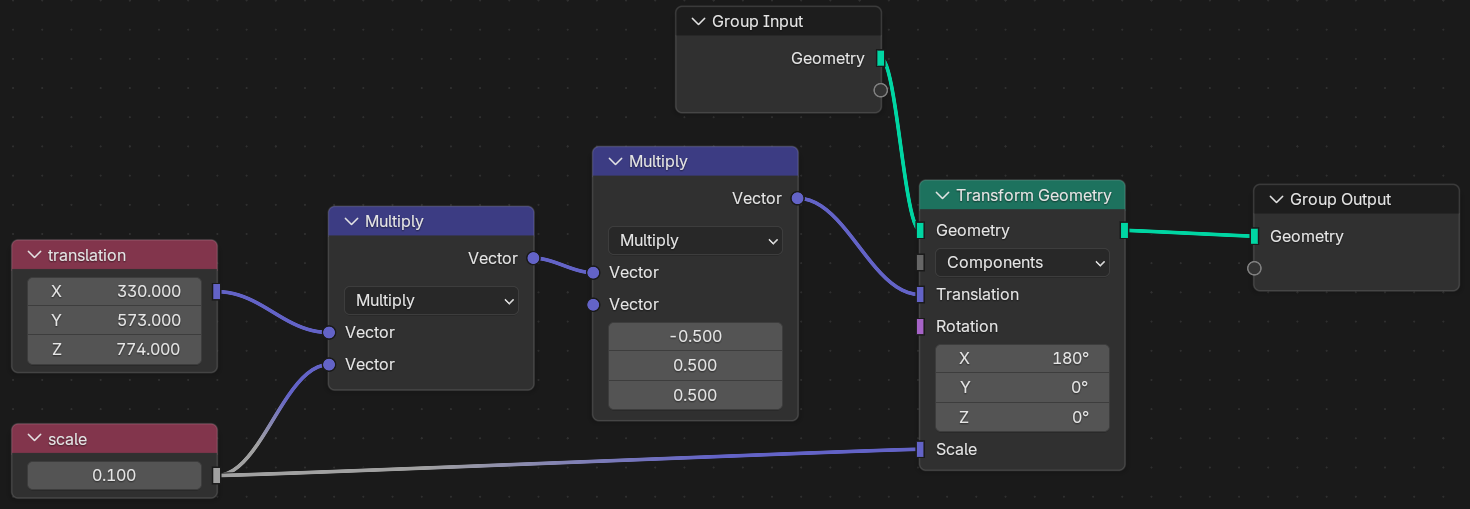
\includegraphics[width=\textwidth]{assets/blender_geometry.png}
	\caption{Geometry Node наложенный на загруженный в Blender объём}
	\label{fig:blender-geometry}
\end{figure}

Для рендеринга используется движок, реализующий трассировку путей --- Cycles. В качестве его параметров, отличных от стандартных выставлено количество отражений внутри объёма, равное 4. Параметры камеры:
\begin{itemize}
	\item Фокусное расстояние: 36 мм;
	\item Размер сенсора: $24\times36$ мм (разрешение $800\times1200$ пикселей);
\end{itemize}

Для обучения 3DGS отрендерено 700 изображений с разных камер, удаленных от центра сцены на 100 метров Blender, перед каждым новым изображением камера размещается на случайной точке сферы, для этого выделены 2 равномерно распределенные случайные величины:
%
\[
	\cos(\phi) \sim U[-1, 1], \text{ где } \phi \text{ - угол, образуемый с } Oz,
\]
\[
	\theta \sim U[0, 2\pi], \text{ где } \theta \text{ - угол в плоскости } Oxy.
\]
%
Скрипт (листинг \ref{lst:blender}) поддерживает создание изображений за несколько сессий, при последующих запусках новые рендеры будут дополнять предыдущие. Также скрипт сохраняет все параметры камеры в файлах, соответствующих формату COLMAP. Пояснения по отличию этих данных от Blender формата приводятся в следующем разделе.

Рендер каждого кадра на видеокарте RTX 2060 с 6 гигабайтами видеопамяти на CUDA бекенде занимал от 3:00 до 3:15 минут, поэтому всего потребовалось чуть больше 35 часов на рендер всего. Далее также будет рассмотрено возможно ли сократить число изображений без потери качества итоговой 3DGS модели.